\chapter{Speichersysteme in Videospielen}\label{ch:videospiele}
Anschauen, wie Videospiele Daten speichern und laden\dots
%--------------------------------------------------------------------------


%--------------------------------------------------------------------------
\section{Minecraft}
Minecraft ist ein Sandbox-Spiel\footnote{Ein Sandbox-Spiel lässt Spieler frei entscheiden, was mit der Spielwelt gemacht werden soll. Es gibt keine feste Geschichte im Spiel, die verfolgt werden muss.\cite{ocio2009multi}}, welches von Mojang Studio entwwickelt wurde. Minecraft gilt unter den meistverkauften Videospiele aller Zeiten und kann auf eine Vielzahl von Plattformen gespielt werden.\cite{ignBestSellingVideo} Es wird in einer dreidimensionalen Welt, die aus Blöcken besteht, gespielt und es kann mit Entitäten interagiert werden. Es gibt verschiedene Spielmodi, wie zum Beispiel ein Überlebens- und Kreativmodus. Beim Überlebensmodus geht es hauptsächlich um das Überleben in der Spielwelt, jedoch kann der Spieler frei entscheiden, was er in der Spielwelt machen wird.\cite{minecraftWikiHome}

\wichtig{Quelle mit Email nennen}

In diesem Kapitel wurde die Minecraft Version 1.16 angeschaut. 
Bei neueren Versionen kann das Speichersystem bereits etwas anders aussehen. Um an den Sourcecode zu kommen wurde das Tool 
\url{https://github.com/Hexeption/MCP-Reborn/tree/1.16} verwendet. Aus rechtlichen Gründen darf kein
Sourcecode gezeigt werden.

\subsection{Daten}
Bevor sich das Speicher- und Ladesystem von Minecraft genauer angeschaut werden kann, ist es erstmal wichtig zu wissen, mit welchen Arten von Daten Minecraft arbeitet. Die Spielwelt in Minecraft besteht aus verschiedenen Blöcken, \wichtig{Entitäten} und Items. 

\textit{Blöcke} werden in Minecraft nicht einzeln behandelt, sondern als Section, ein Bereich von 16x16x16-Block, gespeichert. Mehr zu dieser Aufteilung bei Minecraft gibt es im Abschnitt \ref{ssec:datenaufteilung}. Informationen, die zu so einem Block gehören, sind die Position, BlockID, Block Zustände und Informationen zum Licht. Die Position eines Blocks wird in der Reihenfolge y-, z- und x-Koordinate gespeichert, für bessere Komprimierung. Jeder Blocktyp hat eine eigene BlockID, die diesen Block genau identifiziert. Der Zustand eines Blocks wird für jede Section in einer Liste namens "BlockStates" abgespeichert. Informationen dessen Zustands können zum Beispiel sein, in welcher Himmelsrichtung der Block plaziert wurde, welche Rotation der Block hat und ob der Block am brennen ist. Welche Zustände ein Block haben kann, hängt auch von dem Blocktyp ab.\cite{minecraftBlockStates} Bei den Informationen zum Licht jedes Blocks gibt es für jede Section zwei Listen namens "BlockLight" und "SkyLight". "BlockLight" speichert wieviel Licht jeder Block ausstrahlt und "SkyLight" wieviel jeder Block an Licht abbekommt. Zusätlich gibt es noch sogenannte Block Entitys, die aber nichts mit den Entitäten des Spieles zu tun haben. Diese Speichern zusätliche Informationen zu einem Block, die in der "BlockStates"-Liste nicht gespeichert werden konnten.\cite{minecraftChunkFormat}
%Weitere Quelle: ChunkSerializer.java:write()

Eine Entität kann ein Spieler, ein Tier oder Monster sein. Die wichtigste Information einer Entität ist die Position, Geschwindigkeit und Rotation dieser. Des weiteren gibt es viele weitere Informationen zu einer Entität, wie die Luft die die Entität noch übrig hat zum Überleben, die Distanz die eine Entität schon gefallen ist oder wie lange eine Entität noch brennen wird.\cite{minecraftEntityFormat}
%Weitere Quelle: Entity.java:writeWithoutTypeID()


\textit{Items} bei Minecraft existieren im Inventar, in Kisten, in Item Frames oder in Armor Stands \wichtig{(Englisch)}. Wenn ein Spieler ein Item fallen lässt, dann werden diese als Entitäten in die Welt platziert und als solche gespeichert. Manche Items können in die Welt platziert werden und werden dann zu neuen Blöcken oder Entitäten. Jedes Item hat die Information "Count", "Slot", "id" und "tag". "Count" und "Slot" definieren, wieviele Items in welchem Inventarplatz liegen. Jedes Item hat dabei eine eigene Identifikationsnummer, mit der diese gespeichert werden. "tag" gibt noch zusätliche Informationen über ein Item, wie die Haltbarkeit oder ob ein Item unzerbrechlich ist.
\cite{minecraftPlayerdatFormat}
\cite{minecraftItem}

%Item werdeb z.B. in player.dat gespeichert

\subsection{Ordnerstruktur}
Ordner:
\begin{itemize}
    \item /world/data
    \item /world/players: Player Data
    \item /world/DIM-1: Nether world
    \item /world/DIM1: End world
    \item /world/region: Overworld regions
    \item /world/DIM-1/region: Nether regions
    \item /world/DIM1/region: End regions
\end{itemize}

Dateien:
\begin{itemize}
    \item level.dat: Allgemeine Spieldaten (NBT Struktur)
    \item $[$playeruuid$]$.dat: Spielerdaten
    \item $[$region$]$.mca: Regionen in /region Ordner
\end{itemize}

% 1.8.2023
\url{https://wiki.vg/Map_Format}\\
\url{https://minecraft.fandom.com/wiki/Java_Edition_level_format}

\subsection{Speicherformate}
\begin{itemize}
    \item Minecraft Anvil (MCA): Speichern von Chunk Daten (RegionFileCache.java:loadFile(), SaveFormat.java:convertRegions())
    \item Named Binary Tag (NBT): .dat-Endung $\Rightarrow$ level.dat, Playerdata, ... (CompoundNBT in vielen Dateien und NBT Folder)
    \item JavaScript Object Notation (JSON): Speichern von Texte (Bücher, Schilder, Label)
\end{itemize}

% 1.8.2023
\url{https://docs.fileformat.com/game/mca/}\\
\url{https://wiki.vg/NBT}\\
\url{https://minecraft.fandom.com/wiki/JSON}

NBT:
\begin{itemize}
    \item Zum Speichern von Entitäten oder Blöcken
    \item NBT Objekte werden zu SNBT (stringified NBT) gewandelt um in Speicher zu schreiben 
    \item NBT File = zipped compound tag mit Namen und tag ID 
    \item Zipping mit GZip/zlib
    \item level.dat, $<$player$>$.dat, idcounts.dat, villages.dat, raids.dat, map$\_$$<$\#$>$.dat, Chunks, \dots sind komprimiert im NBT Format gespeichert
    \item servers.dat, hotbar.nbt sind unkomprimiert im NBT Format gespeichert
\end{itemize}
% 1.8.2023
\url{https://minecraft.fandom.com/wiki/NBT_format}

\subsection{Datenaufteilung} \label{ssec:datenaufteilung}
Jedes Level hat seinen Ordner, in dem eine level.dat Datei ist und Ordner um Maps und Regions von diesem Level abzuspeichern. 

\begin{itemize}
    \item Section: Bereich von 16x16x16-Blöcken
    \item Chunk: Bereich von 16x16x$[$Welt Höhenlimit$]$ Blöcken (Bei Minecraft 1.16 Höhenlimit = 256 $\Rightarrow{}$ Chunk = 16xSections (Chunk.java:sections))
    \item Region: Gruppierung von Chunks in einem 32x32 Blöcke Gebiet
    \item Level: (Theoretisch, aber nicht praktisch) unendliche Sammlung von Chunks gespeichert als regions
\end{itemize}

level.dat:
\begin{itemize}
    \item Globale Informationen über der Welt (Uhrzeit, Singleplayer Spieler, seed, \dots)
    \item NBT File
    \item level.dat$\_$old als Backup
\end{itemize}

% 1.8.2023
\url{https://minecraft.fandom.com/wiki/Chunk_format}
\url{https://wiki.vg/Region_Files}
\url{https://minecraft.fandom.com/wiki/Java_Edition_level_format}

\subsection{Speichervorgänge}

Speicherung, wenn:
\begin{itemize}
    \item Neue Welt generiert (Minecraft.java:createWorld())
    \item Pause-Taste wird gedrückt (IntegratedServer.java:tick())
    \item Chunks werden entladen (Spieler zu weit weg)
    \item Alle 5 Minuten
\end{itemize}

% 1.8.2023
\url{https://minecraft.fandom.com/de/wiki/Spielstand-Speicherung}

\subsection{Ladevorgänge}
%--------------------------------------------------------------------------



%--------------------------------------------------------------------------
\section{Factorio}
\begin{enumerate}
    \item Ressourcen minen 
    \item Technologien forschen
    \item Infrastruktur aufbauen
    \item Automatisieren von Produktion
    \item Gegner bekämpfen
    \item In Lua geschrieben
\end{enumerate}
\url{https://www.factorio.com/}

Allgemein benutzt Factorio ein "Deterministic save load"
\url{https://gist.github.com/Rseding91/a309cf0a30782a2e96ef081c39326f42}

\wichtig{Quelle mit Email nennen}

\subsection{Daten}

\begin{figure}[htp]
    \centering
    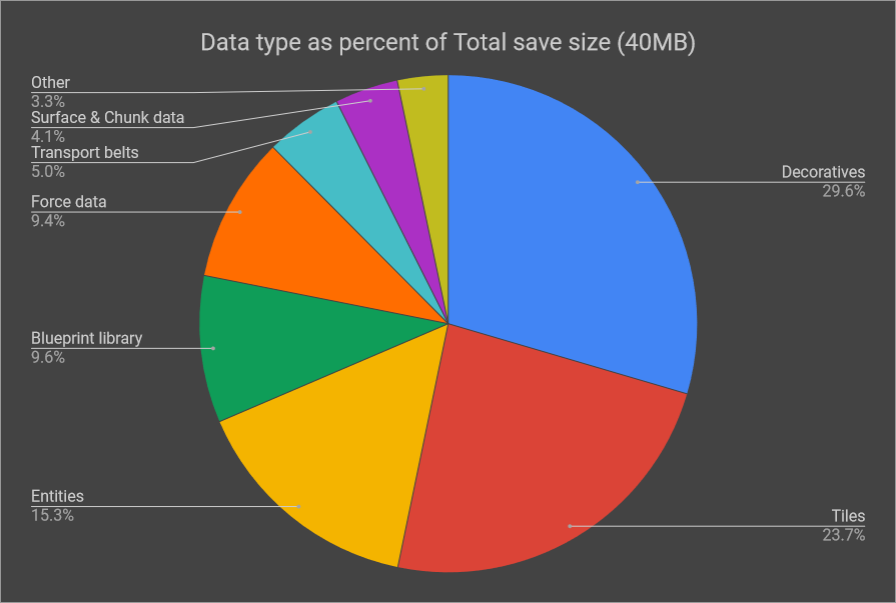
\includegraphics[width=0.8\textwidth]{images/factorio_save_statistic.png}
    \caption{Anteil der Datentypen beim Speichern}
    \label{fig:factorioSaveStatistic}
\end{figure}
% 27.7.2023
\url{https://www.factorio.com/blog/post/fff-270}

Map Daten bestehen aus:
\begin{itemize}
    \item Dekorative Spielobjekte 
    \item Tiles 
    \item Entitäten
    \item Blueprint Library
    \item Physikalische Kräfte
    \item Transportband
    \item Oberfläche und Chunk Daten
    \item Weitere Daten...
\end{itemize}

\subsection{Ordnerstruktur}
User data Ordner:
\begin{itemize}
    \item ./saves (Save files)
    \item ./mods (Mods)
    \item ./script-output (Script-output, z.B. von Spiel Screenshots)
    \item ./scenarios (Lokale Szenarien)
    \item ./config/config.ini (Lokale Einstellung)
    \item factorio-*.log (Log files)
    \item factorio-dump-*.dmp (Crash dump files)
\end{itemize}

%2.8.2023
\url{https://wiki.factorio.com/Application_directory} %Offizielle Factorio Wiki laut Seite

\subsection{Speicherformate}

\subsection{Datenaufteilung}

\subsection{Speichervorgänge}
Kurzgefasst:
\begin{enumerate}
    \item ID Mapping speichern (\url{https://www.factorio.com/blog/post/fff-259}) %2.8.2023
    \item Map Daten speichern
\end{enumerate}

Detaillierter:
\begin{enumerate}
    \item Volles leeren der Garbage Collection von allen Lua Zuständen
    \item Löschen von temporären Map Daten, die während des Speicherprozesses entstanden sind
    \item ID mapping speichern (ID mapping für alles was IDs benutzt)
    \item Speichern der Prototypenmigrationen
    \item Rest, der gespeichert weden soll, abspeichern
    \item SaveHelpers speichern
\end{enumerate}
%2.8.2023
\url{https://gist.github.com/Rseding91/a309cf0a30782a2e96ef081c39326f42} 

\subsection{Ladevorgänge}
Kurzgefasst:
\begin{enumerate}
    \item Map Version überprüfen
    \item Überprüfen ob Mods hinzugefügt/gelöscht/verändert wurden
    \item invalide/korrupte save files finden 
\end{enumerate}

Detaillierter:
\begin{enumerate}
    \item Map-Version überprüfen (save file map und die map in der die save file map geladen wird)
    \item Überprüfen, ob aktive Mods oder die Mod-Einstellungen sich verändert haben (wenn ja, müssen Aktionen nach dem laden durchgeführt werden) und setze flag wenn das der Fall ist
    \item ID mapping laden
    \item Angewandte Migrationen laden und nicht angewandte Migrationen ausführen
    \item Standard Map Daten laden (Enitäten, Chunks, Forces, Züge)
    \item load in allen LoadHelpers aufrufen
    \item Inszenierte (???) Veränderungen ausführen
    \item Enitäten, die Ladeprobleme hatten, nachladen
    \item Targeters wiederherstellen
    \item setup bei allen LoadHelpers ausrufen
    \item Wenn Prototyp Daten verändert wurden Elektrisches Netz Daten clearen
    \item setup aller transport belt connectible Entitäten aufrufen
    \item Ruf setup von Entität auf, wenn diese während Laden erstellt wurde und nicht existierte, als die Map zuletzt gespeichert wurde
    \item postLoadHook für die Map aufrufen
    \item Tile Probleme fixen, nachdem alle Enitäten geladen wurden und setup fertig ist
    \item Ruf bei allen PreFinalLoadHelper setup auf
    \item Ruf bei allen FinalLoadHelper setup auf
    \item Für alle Oberflächen postSetup aufrufen
    \item Lua Daten laden und wiederherstellen
    \item "configuration changed" Lua event ausführen
\end{enumerate}
%--------------------------------------------------------------------------

\iffalse
%--------------------------------------------------------------------------
\section{Terraria}
\subsection{Daten}
Welche Klassen gibt es bei Terraria (Blöcke, Chunks,...) und welche Daten 
beinhalten diese.

\subsection{Ordnerstruktur}

\subsection{Speicherformate}
World-Dateien, Player-Dateien, Konfigurationsdateien 

\subsection{Datenaufteilung}
Kein Chunksystem, alles in einer Datei gespeichert. Aber Inventar, Position
usw. werden in verschiedenen Daten gespeichert.

\subsection{Speichervorgänge}

\subsection{Ladevorgänge}
%--------------------------------------------------------------------------


%--------------------------------------------------------------------------
\section{Ein Spiel}
Beschreibung von dem Spiel

\subsection{Daten}
Welche Klassen gibt es bei <Spielname> (Blöcke, Chunks,...) und welche Daten 
beinhalten diese.

\subsection{Ordnerstruktur}

\subsection{Speicherformate}

\subsection{Datenaufteilung}

\subsection{Speichervorgänge}

\subsection{Ladevorgänge}
\fi
